\section{Decentralized search for \\ shortest path approximation}
\label{searching}

In this section, we are going to discuss how to perform decentralized searches based on the index structures to achieve a higher accuracy. We will also discuss how to optimize and control the search space of decentralized search to maintain low online search overheads.

\subsection{Index guided decentralized search}

\begin{figure}[t]
    \centering
    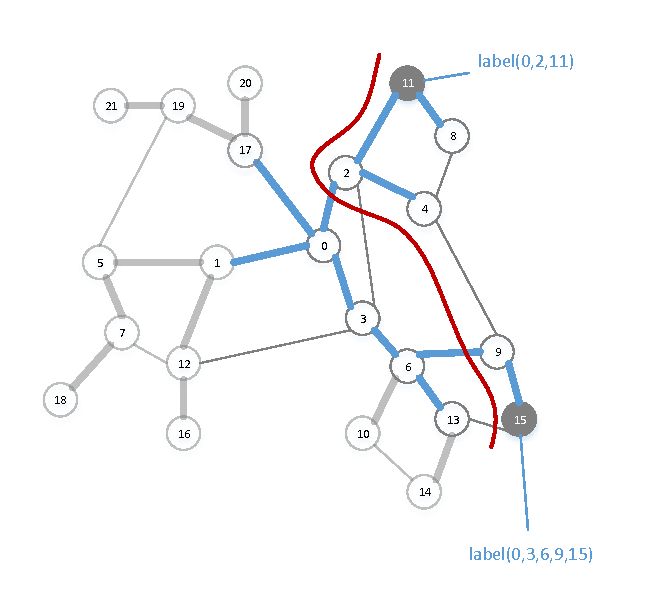
\includegraphics[width=\linewidth]{./figures/new_illustrate/dec_common.pdf}
    \caption{Decentralized search explores the edges that are not directly connected to the indexed shortest path. Edge $(4, 9)$ cannot be found by solely searching circles in the path by LCA distance.}
    \label{fig:dec_common}
\end{figure}

We perform decentralized search on an indexed graph as follows. For a given pair of source and target vertex, the search start at the source vertex and set it as the currently visited vertex and append it to the approximated path. The search examines each neighbor of currently visited vertex, for each neighbor, the LCA distance to the target vertex is calculated. The neighbor with least LCA distance will be picked as the vertex to visit next and append it to the approximated path. This step continues until the search reach the target vertex. The algorithm is depicted in \ref{alg:dec}.

\begin{algorithm}
    \caption{Algorithm decentralized search}
		\label{alg:dec}
    \begin{algorithmic}
        \Function{DecentralizedSearch}{$G$, $s$, $t$}
					\State $p_{appr.} \gets \emptyset$
					\State $u \gets s$
					\State $p_{appr.} = p_{appr.} \cup u$
					\While{$u \neq t$}
						\State $d_{min} \gets \infty$
						\State $w \gets u$
						\For{$each v adjecent to u$}
							\If{$d_{LCA}(v,t) < d_{min}$}
								\State $d_{min} \gets d_{LCA}(V,t)$
								\State $w \gets v$ 
							\EndIf
						\EndFor
						\State $u \gets w$
						\State $p_{appr.} = p_{appr.} \cup u$
					\EndWhile
					\State \Return $p_{appr.}$
        \EndFunction
    \end{algorithmic}
\end{algorithm}

By calculating the LCA distance to the target from each neighbor, the search can explore edges that do not contained in the indexes. By choosing the neighbor with least LCA distance, the search does not constrained itself to vertices in the label of source and target vertices. For example in Fig. \ref{fig:dec_common} from $15$ to $11$, by following the procedure of decentralized search, instead of finding a edge with both ends in labels of vertex $15$: $(0, 3, 6, 9, 15)$ and $11$: $(0, 2, 11)$, our approach find a edge $(9, 4)$ that can lead to a shorter path which is denoted by solid curved line. 

As long as the source vertex $s$ and target vertex $t$ are reachable from each other, decentralized search will terminate in as much as $2 * max_{u,v}d_G(u,v)$ steps, where $max_{u,v}d_G(u,v)$ is the diameter of the network. Too see this, for the LCA distance of an arbitrary pair of source and target vertex $s$ and $t$, the following bound holds:

\begin{equation}
\label{equ:term}
\begin{split}
    d_{LCA}(s,t) \leq max_{l \in L}\{d_G(s,c_l(s,t)) + d_G(c_l(s,t),t)\} \\
		\leq max_{u,v}d_G(u,v) + max_{u,v}d_G(u,v)
\end{split}
\end{equation}

And at each step, suppose decentralized search is visiting vertex $p$, there is a neighbor of vertex $q$ that is on the path indicated by LCA computation of $p$ and $t$ we denoted as $q$. We have $d_{LCA}(q,t) \leq d_{LCA}(p,t) - 1$. Since decentralized search always pick the neighbor with least LCA distance to the target, the LCA distance to the target at each step will decrease at least by $1$. Therefore, decentralized search will terminate in at most $d_{LCA}(s,t)$ steps. According to equation \ref{equ:term}, decentralized search for arbitrary pairs of reachable vertices will terminate in at most $2 * max_{u,v}d_G(u,v)$ steps.

However, terminating when the search reaches the target vertex is a valid but not an ideal stopping criterion. Since the label of each vertex stores the shortest path of each vertex to each landmark. And shortest path follows the optimal substructure, i.e. the path between any two vertices along the shortest path is also the shortest path of them. So a better terminate condition is to stop the search when reaching any vertex in the label of the target vertex. Since the path contained in the label of target vertex is already the the shortest path from this vertex to the target vertex due to the optimal substructure, we can directly concatenate it to the visited vertices to form a approximated path. With this terminate condition, required step for decentralized search is reduced from at most $2 * max_{u,v}d_G(u,v)$ to at most $max_{u,v}d_G(u,v)$. 

The time complexity of Decentralized search depends on the several parameters of the graph. Decentralized search take $O(max_{u,v}d_G(u,v))$ steps to finish. For each step, the search need to check $O(max_{u}Degree(u))$ neighbors. For each neighbor, $k$ LCA computations are required where $k$ is the number of landmarks. Each LCA computations only takes constant times $O(1)$. So the time complexity of decentralized search depends on the average degree and the diameter of the graph. For Space complexity, first the landmark embedded in every node takes $O(kn)$ space. For each query, only $O(k)$ space is required to store the labels of target vertex and the vertex that is being examined.

\subsection{Bi-directional search}

\begin{figure}[t]
    \centering
    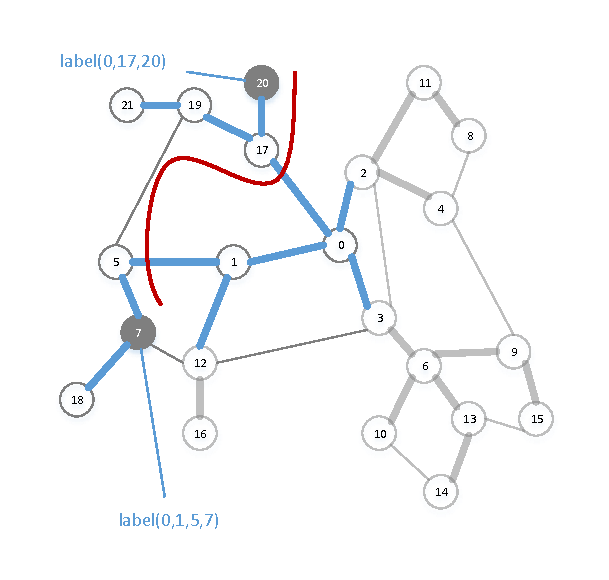
\includegraphics[width=\linewidth]{./figures/new_illustrate/bi_dec.pdf}
    \caption{Bidirectional decentralized search can explore different set of edges which may found path at different length. Searches start at vertex $7$ will lead to a path shorter than starting at $20$ by taking advantage of the edge $(5, 19)$.}
    \label{fig:bi_dec}
\end{figure}

In this section we show how to combine the bidirectional search and decentralized search together. Unlike bidirectional BFS, the goal for performing bidirectional search is not to reduce search space but to increase accuracy. A reversed search starting at target vertex and aim at source vertex may explore a different set of vertices and edges which may lead to a different path, sometimes with shorter length, to be found compared to the original search. For example in Fig. \ref{fig:bi_dec}, the search starts from $20$ to $7$ can find a shorter path $p = (20, 17, 19, 5, 7)$ than the search starts at $7$. Due to that $0$ has a smaller LCA distance to $7$ than $19$, the edge $(19, 5)$ cannot be found by the search starts from $20$. 

In BFS, we expect two search will meet in some intermedia vertices that can be used as a new stop criterion which lead to reduced search space. But in decentrailzed search, there is no guarantee that two search will meet at any vertex except the source/target vertex. Since two search are driven by two distinct goals: finding next hop with least LCA distance to source/target vertex. 

[explained by an example]

\subsection{Handle ties}

\begin{figure}[t]
    \centering
    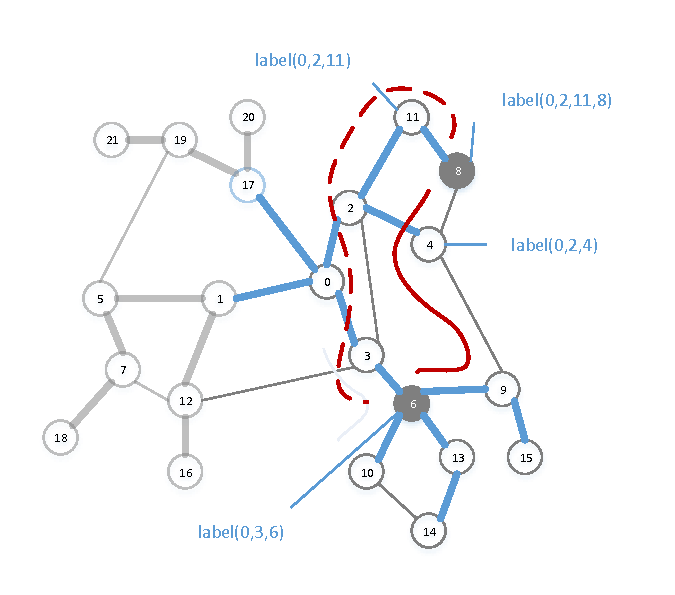
\includegraphics[width=\linewidth]{./figures/new_illustrate/tie.pdf}
    \caption{Tie happens during decentralized search. Although LCA distances are the same, selecting different neighbor will search different part of the graph which may lead to paths at different length.}
    \label{fig:tie}
\end{figure}

Tie happens frequently in decentralized search especially when the number of landmark is small. The tie here means during a step when decentralized search examining neighbors of currently visited vertex, there is not sufficient information in the index that can separate several neighbors, i.e. they have the same LCA distance to the target. For example in Fig. \ref{fig:tie}, to find path from $8$ to $6$, when traversing neighbors of vertex $8$, both vertex $11$ and $4$ have the same LCA distance to vertex $6$, but their actual distances to vertex $6$ are different due to edges currently invisible to the decentralized search. Labels of each neighbor, on the other hand, provide no clue which one can lead to a shorter path.

Expanding the search onto each tie vertex require the search examine different sets of vertices and edges which will increase the cost of the search, but will increase the chance to find a shorter path as well. So two obvious solution to deal with ties are either randomly pick one vertex to visit or visit all vertices in the next step. The former one incur no additional cost and will have the least possibility to find a shorter path. The latter one require most effort and will lead to the shortest path the decentralized search could find.

[the lca heuristic and effort/shorter path ratio.]
